% Chapter Template

\chapter{Ensayos y resultados} % Main chapter title

\label{Chapter4} % Change X to a consecutive number; for referencing this chapter elsewhere, use \ref{ChapterX}

En este capítulo se describe la estrategia de pruebas adoptada para determinar que el sistema se comporta de forma esperada.

%----------------------------------------------------------------------------------------
%	SECTION 1
%----------------------------------------------------------------------------------------

\section{Laboratorio remoto}
\label{sec:lab}

Durante las primeras etapas del desarrollo no se disponía en Buenos Aires del dispositivo bajo prueba.
Por esta razón, se montó un laboratorio remoto en San Carlos de Bariloche.
Se dispuso una placa de evaluación \emph{SAM V71 Xplained Ultra} conectada a un ordenador dentro de la red de INVAP S.E.
La conexión entre la placa y el ordenador se logró a través de una sonda de depuración \emph{Segger J-32}.

Para poder acceder al laboratorio remoto que se muestra en la figura \ref{fig:remotelab} se necesitó:

\begin{itemize}
    \item Credenciales de acceso y conexión a la VPN de INVAP S.E.
    \item Crear un túnel SSH con el ordenador remoto.
\end{itemize}

El túnel SSH se generó con \emph{X11 forwarding} habilitado.
De esta manera, se pudo generar ventanas gráficas en el ambiente local.
Además, las operaciones de consola se integraron al ordenador personal con una sesión de Tmux.
Finalmente, se logró implementar una interfaz de control del laboratorio remoto con una apariencia idéntica al ambiente local.

\begin{figure}[htbp]
	\centering
	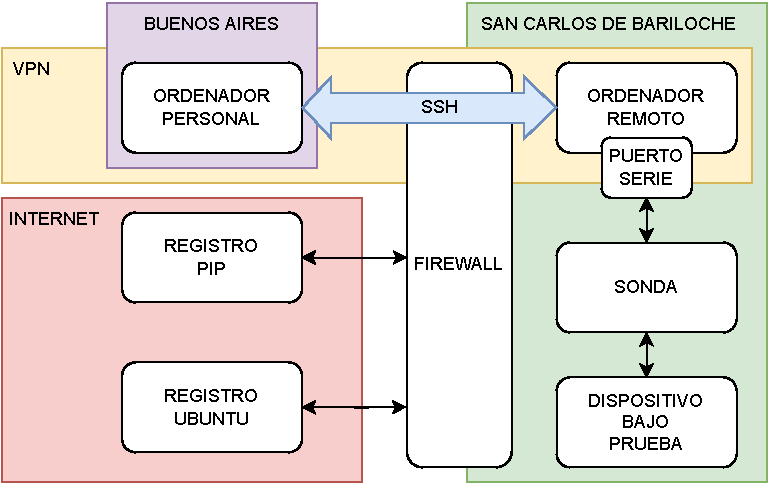
\includegraphics[width=\textwidth]{./Figures/vpn.pdf}
    \caption{Diagrama en bloques del laboratorio remoto.}
	\label{fig:remotelab}
\end{figure}

Para poder instalar las dependencias y los servidores OCD evaluados, se habilitaron los puertos necesarios que permitieron al ordenador remoto conectarse a los recursos en la Internet.
Sin embargo, algunos recursos debieron ser compilados en el \emph{host} y la transferencia de los \emph{tarballs} se realizó por medio de \emph{Secure Copy Files (SCP)}.

Con el laboratorio remoto montado, se procedió a realizar las siguientes pruebas:
\begin{itemize}
    \item Pruebas de configuración de sondas de depuración y compatibilidad con servidores OCD.
    \item Pruebas de acceso al dispositivo bajo prueba.
\end{itemize}

Las pruebas referidas a la sonda de depuración arrojaron como resultado lo siguiente:

\begin{itemize}
    \item El modo de \emph{boot} de la sonda determina el nivel de acceso al dispositivo bajo prueba.
    \item Para lograr inyecciones de \emph{soft-errors} la sonda de depuración debe poder iniciar en modo \emph{CMSIS-DAP}.
    \item Si la sonda de depuración no se encuentra en modo \emph{CMSIS-DAP}, \emph{PyOCD} solo puede realizar escritura en la memoria \emph{flash}.
    \item Cambiar de modo una sonda de depuración requiere reiniciarla.
        Por lo tanto, no es factible realizar cambios de configuración luego de iniciado un ensayo.
\end{itemize}

Las pruebas referidas al acceso al dispositivo bajo prueba tuvieron los siguientes resultados:

\begin{itemize}
    \item Si no se dispone de un \emph{Device Family Pack (DFP)}, \emph{PyOCD} se conecta al dispositivo bajo prueba y lo identifica como \emph{Generic Cortex-M}.
    \item Bajo la identificación de \emph{Generic Cortex-M} se puede acceder a todos los registros de núcleo.
    \item Bajo la identificación de \emph{Generic Cortex-M} se puede acceder a la memoria \emph{SDRAM} y reconoce como error una posición desalineada.
    \item Bajo la identificación de \emph{Generic Cortex-M} se puede acceder a otras direcciones del integrado solo en modo lectura.
        Si se intenta ingresar en modo escritura no sucede ningún cambio pero el servidor OCD no responde con un error.
        Su respuesta es de operación exitosa, pero no se manifiestan cambios.
\end{itemize}

PyOCD posee un módulo de búsqueda y descarga de DFP, sin embargo, su funcionamiento no es confiable y genera una excepción durante su ejecución.
Se intentó verificar su funcionamiento en otras plataformas y se pudo observar que su desarrollo fue realizado en el lenguaje de programación \emph{Rust}.
Este módulo hizo imposible instalar el servidor OCD en una \emph{single board computer}.
Dado que, su compilador consume una cantidad de memoria que supera el \emph{hardware} disponible en placas como \emph{Raspberry Pi 4B}.
Se pudo verificar que este es el único módulo escrito en \emph{Rust}, pero no es posible desacoplarlo del servidor OCD.
Finalmente, PyOCD tiene una limitación de plataformas compatibles que podría ser sorteada con \emph{cross} compilación.

La única dificultad en el uso del laboratorio remoto se presentó en las pruebas de la sonda de depuración.
Muchas de las pruebas requirieron reiniciar la sonda y esto solo es posible al desconectar el cable \emph{USB}.
La operación debió ser realizada por el co-director de este trabajo.

En la tabla \ref{tab:funcionalidades}, se puede ver un resumen de las funcionalidades del laboratorio remoto.
Las funcionalidades con tres marcas tienen el mismo nivel de servicio que el laboratorio local, las de dos marcas tienen un nivel algo inferior y las que tienen solo una marca tienen un nivel de servicio bajo.

\begin{table}[h]
	\centering
	\caption[Resumen del laboratorio remoto]{Resumen del laboratorio remoto.}

	\begin{tabular}{l c}    
		\toprule
        \textbf{Funcionalidad}             & \textbf{Nivel de servicio} \\
		\midrule
		Carga de binarios en DUT           & ++  \\		
		Comunicación con registro PIP      & +++ \\
		Comunicación con registro Ubuntu   & +++ \\
		Comunicación con debug access port & +++ \\
		Comunicación con UART              & +   \\
		\bottomrule
		\hline
	\end{tabular}
	\label{tab:funcionalidades}
\end{table}

\section{Ensayos de inyector}
\label{sec:testinyector}

El inyector de \emph{soft-errors} se sometió a ensayos en los siguientes ambientes:

\begin{itemize}
    \item Laboratorio remoto.
    \item Laboratorio local.
    \item Dispositivo alternativo \emph{NUCLEO-F429ZI}.
        Este último ambiente se puede ver en la figura \ref{fig:alternativo} y se utilizó para probar si el inyector es genérico.
        En particular, porque utiliza una sonda de depuración distinta.
\end{itemize}

\begin{figure}[htbp]
	\centering
	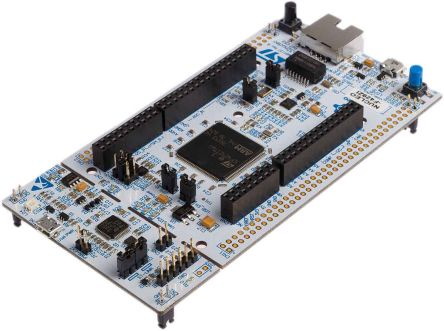
\includegraphics[width=0.8\textwidth]{./Figures/alternativo.jpg}
    \caption{Dispositivo alternativo \emph{NUCLEO-F429ZI}.}
	\label{fig:alternativo}
\end{figure}

Se generaron múltiples archivos de configuración para definir distintos casos de prueba.
Luego, se corrieron los ensayos en los tres ambientes y se compararon los resultados.
Además, se usó una variante adicional en el dispositivo alternativo.
Se probó el comportamiento del inyector sobre un blanco con \emph{mbedOS}.
Finalmente, en la tabla \ref{tab:resensayos} se puede observar un resumen de los resultados obtenidos.

En la tabla se marca con tres cruces los ensayos que arrojaron resultados sobresalientes, con dos cruces los ensayos que mostraron inconvenientes mínimos y con una cruz los ensayos con resultados insatisfactorios.

\begin{table}[h]
	\centering
	\caption[Resumen de ensayos]{Resumen de ensayos.}

	\begin{tabular}{l c c c}    
		\toprule
        \textbf{Ensayo}                 & \textbf{Lab. local} & \textbf{Lab. remoto} & \textbf{DUT alterno} \\
		\midrule
		Escritura SDRAM                 & +++                 & +++                  & +++ \\
		Escritura registros CORE        & +++                 & +++                  & +++ \\
		Funcionalidades extras          & ++                  & ++                   & +++ \\
		Halt CORE                       & +++                 & +++                  & +++ \\
		Lectura SDRAM                   & +++                 & +++                  & +++ \\
		Lectura registros CORE          & +++                 & +++                  & +++ \\		
		Uso concurrente de puerto serie & +++                 & +                    & +++ \\
        Resume CORE                     & +++                 & +++                  & +++ \\
		\bottomrule
		\hline
	\end{tabular}
	\label{tab:resensayos}
\end{table}

El dispositivo alternativo arrojó los mejores resultados porque PyOCD tiene el \emph{Device Family Pack}.
Por otro lado, el laboratorio remoto tuvo malos resultados en las pruebas de concurrencia.
Esto fue así ya que se debía pedir ayuda al personal de INVAP S.E. cada vez que la sonda necesitaba ser reiniciada. 

\section{Validación con el cliente}
\label{sec:validacion}

La etapa final del proceso de pruebas fue una serie de demostraciones realizadas al cliente.
Luego de cada demostración se indicaban las correcciones a realizar.
Seguidamente, se mejoraba el código y se repetía la demostración.
Estos ciclos de iteraciones tenían una frecuencia de 15 días.
Finalmente, se llegó al cumplimiento total de los requerimientos como se puede ver en la tabla \ref{tab:validacion}

\begin{table}[h]
	\centering
	\caption[Resumen de la validación con el cliente]{Resumen de la validación con el cliente.}

	\begin{tabular}{l c}    
		\toprule
        \textbf{Expectativas}     & \textbf{Cumplimiento} \\
		\midrule
		Acceso a memoria          & +++                   \\
		Acceso al CORE            & +++                   \\
		Biblioteca de ensayos     & +++                   \\		
		Capacidad de bit-flip     & +++                   \\
		Configuración del sistema & +++                   \\
		Distribución de errores   & +++                   \\
		Validación de periféricos & +++                   \\
        Generación de reportes    & +++                   \\
		\bottomrule
		\hline
	\end{tabular}
	\label{tab:validacion}
\end{table}

En la figura \ref{fig:demobitflip} se puede observar una demostración del acceso a memoria SDRAM.
Se puede ver que la terminal está dividida en las siguientes partes:

\begin{itemize}
    \item Sección izquierda: se hizo una demostración paso a paso.
        Primero, se importó la biblioteca dentro del espacio de trabajo.
        Luego, se conectó al dispositivo y se cargó una dirección de memoria y el bit a invertir.
        Seguidamente, se realizó una inversión y se mostró el valor previo y posterior al \emph{bit flip}.
        Finalmente, se cerró la conexión con el dispositivo alternativo.
    \item Sección derecha: se observa el mapa de memoria SDRAM del dispositivo alternativo.
        Se usó para mostrarle al cliente las direcciones de memoria ensayadas.
\end{itemize}

Este ensayo además de demostrar el acceso a memoria SDRAM también ejercita la capacidad de realizar \emph{bit flip}.
Finalmente, el cliente consideró que se habían cumplido todos los requisitos y que el trabajo se encontraba finalizado.

Los ensayos finales se volvieron a reproducir en presencia de un estudiante de la especialización en sistemas embebidos quién actualmente utiliza la herramienta en el marco de su proyecto final.

\begin{figure}[htbp]
	\centering
	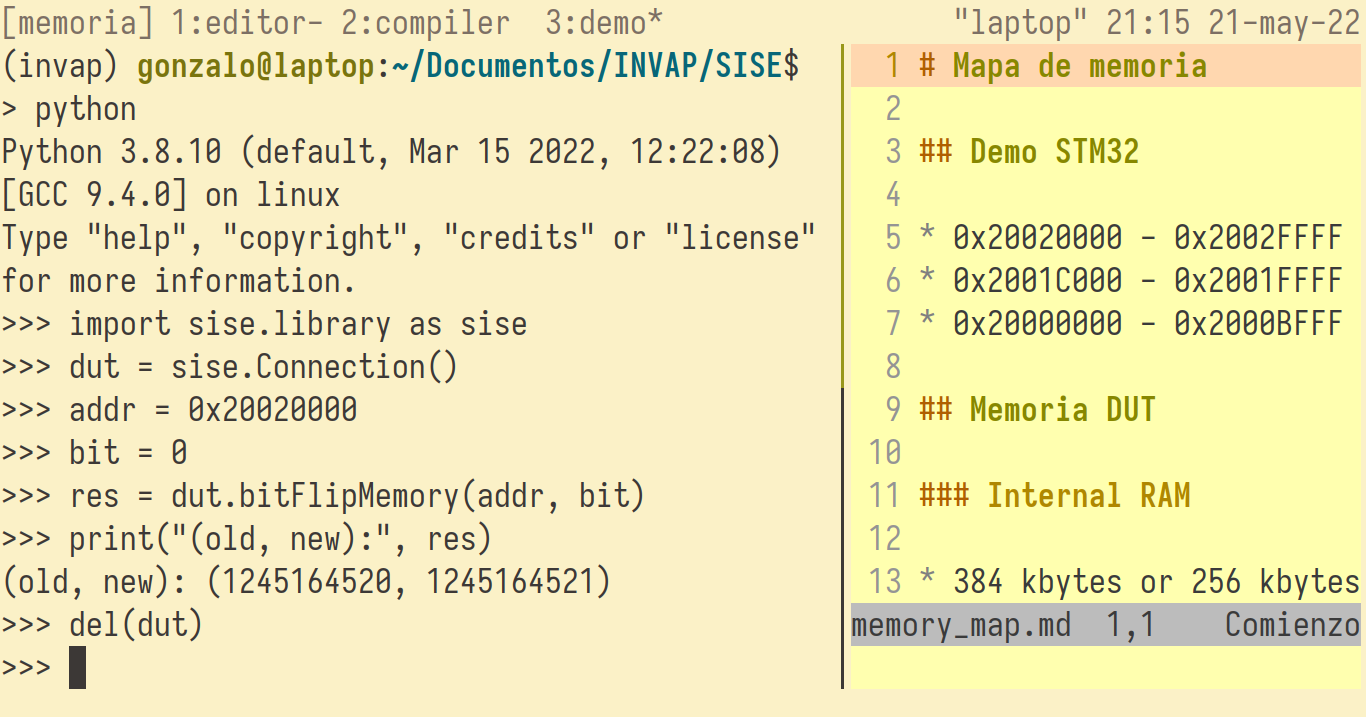
\includegraphics[width=\textwidth]{./Figures/demo_bitflip.png}
    \caption{Demostración de acceso a memoria.}
	\label{fig:demobitflip}
\end{figure}
